\section{Sierpinski Triangle}
\label{sec:SierpinskiTriangle}
\textcolor{gray}{
\lipsum[1-1]
}
\cite{sierpinskiWiki}.

\subsection{Sierpinski triangle by random points}
Sierpinski triangle can be obtained by randomly selected points. 
To draw it in this way one can follow the path below.

\subsubsection{Three corner points of an equilateral triangle}
An equilateral triangle is represented by its corner points first.
\begin{figure}[htb]
\centering
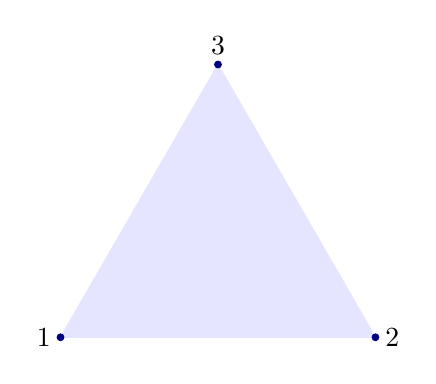
\begin{tikzpicture}
\coordinate (A) at (0,0); 
\coordinate (B) at (4,0); 
\coordinate (C) at (2,3.464);
\draw[fill, blue!10!white] (A) -- (B) -- (C) -- (A);
\draw[fill, blue!50!black] (A) circle (1.2pt) node[black,  left]{$1$};
\draw[fill, blue!50!black] (B) circle (1.2pt) node[black, right]{$2$};
\draw[fill, blue!50!black] (C) circle (1.2pt) node[black, above]{$3$};
\end{tikzpicture}
\caption{An equilateral triangle corner points}
\label{fig:threePoints}
\end{figure}

\subsubsection{Selecting a random point}
Later, a random point is choosen on the triangle.
\begin{figure}[htb]
\centering
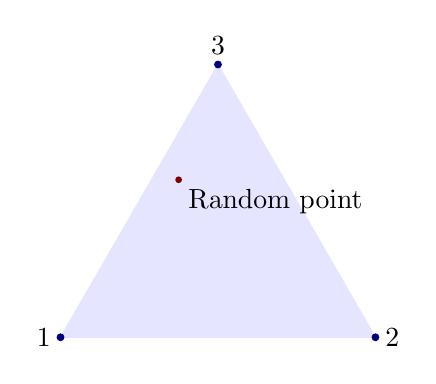
\begin{tikzpicture}
\coordinate (A) at (0,0); 
\coordinate (B) at (4,0); 
\coordinate (C) at (2,3.464);
\draw[fill, blue!10!white] (A) -- (B) -- (C) -- (A);
\draw[fill, blue!50!black] (A) circle (1.2pt) node[black,  left]{$1$};
\draw[fill, blue!50!black] (B) circle (1.2pt) node[black, right]{$2$};
\draw[fill, blue!50!black] (C) circle (1.2pt) node[black, above]{$3$};
\draw[fill, red!50!black] (1.5,2) circle (1pt)  node[black, below right]{Random point};
\end{tikzpicture}
\caption{Random point on the equilateral triangle}
\label{fig:randomPoint}
\end{figure}
\begin{figure}[hb!]
\centering
\begin{tikzpicture}
\node at (0,0.0) {\includegraphics[page=3]{midpoints.pdf}};
\node at (0,4.2) {\includegraphics[page=2]{midpoints.pdf}};
\node at (0,8.4) {\includegraphics[page=1]{midpoints.pdf}};
\end{tikzpicture}
\caption{The first midpoint is selected in the middle of the point $1$ (randomly selected) and the random point (\textit{top}).
The second midpoint is selected in the middle of the point $2$ (randomly selected) and the first midpoint (\textit{middle}).
The third midpoint is selected in the middle of the point $3$ (randomly selected) and the second midpoint (\textit{bottom})}
\label{fig:firstMidPoint}
\end{figure}

\subsubsection{Selecting a midpoint}
In the following step, a corner point is selected randomly and another point is drawn 
in the middle of this corner point and the random point (see Figure~\ref{fig:firstMidPoint}).

\begin{figure}[ht!]
\centering
\begin{tikzpicture}
\node at (0,0.0)  {\includegraphics[page=4]{iterations.pdf}};
\node at (0,4.2)  {\includegraphics[page=3]{iterations.pdf}};
\node at (0,8.4)  {\includegraphics[page=2]{iterations.pdf}};
\node at (0,12.6) {\includegraphics[page=1]{iterations.pdf}};
\end{tikzpicture}
\caption{The points after 10, 100, 1000, and 2000 iterations 
from \textit{top} to \textit{bottom}}
\label{fig:iterations}
\end{figure}
When this process is repeated for 10 times, 
100 times, 
100 times,
1000 times, and
20000 times, Figure~\ref{fig:iterations} is obtained.

\subsubsection{Method}
Figure~\ref{fig:iterations} and other fractal pictures can be obtained with some simple calculations in Python.
There are also some libraries to do it. 
However, an example script can generate the Sierpinski Triangle manually is given in Appendix~\ref{app:sierpinski}.

\textcolor{gray}{
\lipsum[2][1-7]
}

\subsection{Upside down Sierpinski triangle}
Another way of making Sierpinski triangle is explained in the following sections.

\subsubsection{Start with a triangle}
Let's use a upside down equilateral triangle first. 
Then, take its half and recombine three of the half models together to obtain the original shape
(see Figures~\ref{fig:sierpinskiWithSurfaces1},
\ref{fig:sierpinskiWithSurfaces2}, and
\ref{fig:sierpinskiWithSurfaces3}).

\begin{figure}[ht!]
\centering
\begin{tikzpicture}
\coordinate (A) at (0,0); 
\coordinate (B) at (4,0); 
\coordinate (C) at (2,-3.464);
\draw[latex-latex] (0,0.2) -- (4,0.2) node[midway, above]{$l$};
\draw[blue!50!black] (A) -- (B) -- (C) -- (A);

\coordinate (A) at (5,0); 
\coordinate (B) at (6.33,0); 
\coordinate (C) at (5.66,-1.155);
\draw[latex-latex] (5,0.2) -- (6.33,0.2) node[midway, above]{$l/2$};
\draw[blue!50!black] (A) -- (B) -- (C) -- (A);

\draw[latex-latex] (1.3,-3.8) -- (5.3,-3.8) node[midway, above]{$l$};
\node[anchor=north west] at (1.165,-4){\includegraphics{lines1.pdf}};

\end{tikzpicture}
\caption{The upside down equilateral triangle, halved model, and recombined model, from \textit{left} to \textit{right} and \textit{top} to \textit{bottom}}
\label{fig:sierpinskiWithSurfaces1}
\end{figure}


\begin{figure}[hb!]
\centering
\begin{tikzpicture}
\draw[latex-latex] (0.145,0.2) -- (4.145,0.2) node[midway, above]{$l$};
\draw[latex-latex] (5.145,0.2) -- (6.475,0.2) node[midway, above]{$l/2$};
\draw[latex-latex] (1.3,-3.8) -- (5.3,-3.8) node[midway, above]{$l$};
\node[anchor=north west] at (0,0){\includegraphics[page=1]{lines2.pdf}};
\node[anchor=north west] at (5,0){\includegraphics[page=2]{lines2.pdf}};
\node[anchor=north west] at (1.165,-4){\includegraphics[page=3]{lines2.pdf}};
\end{tikzpicture}
\caption{The equilateral triangle at the second step, halved model, and recombined model from \textit{left} to \textit{right} and \textit{top} to \textit{bottom}}
\label{fig:sierpinskiWithSurfaces2}
\end{figure}

\begin{figure}[htb!]
\centering
\begin{tikzpicture}
\node[anchor=north west] at (0,4.2){\includegraphics[page=1]{lines34567.pdf}};
\node[anchor=north west] at (0,0){\includegraphics[page=2]{lines34567.pdf}};
\node[anchor=north west] at (0,-4.2){\includegraphics[page=3]{lines34567.pdf}};
\node[anchor=north west] at (0,-8.4){\includegraphics[page=4]{lines34567.pdf}};
\node[anchor=north west] at (0,-12.6){\includegraphics[page=5]{lines34567.pdf}};
\end{tikzpicture}
\caption{The third, fourth, fifth, sixth, and seventh steps
from \textit{top} to \textit{bottom}}
\label{fig:sierpinskiWithSurfaces3}
\end{figure}

The scripts can be seen in Appendix~X.


